\section{Costos del Sistema}

Finalmente se hace necesario resaltar los costos asociados al desarrollo del controlador estos  se encuentran en el apartado de Anexos (véase \ref{fig:costesDesarrolloControlador}). Se resalta que el costo de los componentes electrónicos y mecánicos fue de alrededor de los \textbf{\$2'000.000}. Cabe resaltar que el desarrollo del controlador incluyendo la etapa de diseño electrónico, diseño mecánico, software, firmware y pruebas llevo alrededor de 350 horas ocasionando que el costo de desarrollo del controlador de vuelo fuera de cerca de los \textbf{\$6'4000.0000} pesos teniendo en cuenta el salario de un ingeniero electrónico promedio en Colombia que es de \textbf{ \$12.664} por hora .  

\begin{figure}[H]
    \centering
    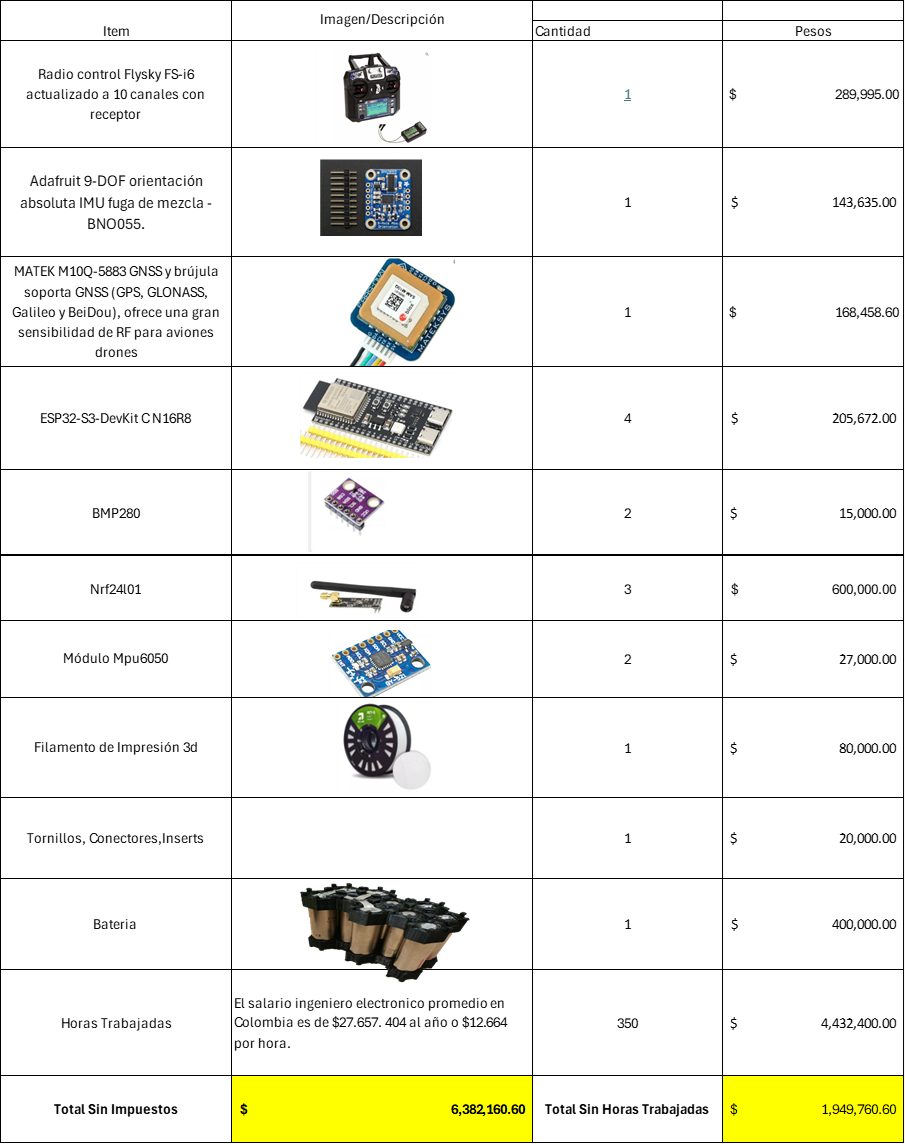
\includegraphics[width=13 cm]{Imagenes/Costos/presupuesto.png}
    \caption{Costos desarrollo Controlador }
    \label{fig:costesDesarrolloControlador}
\end{figure}